% Article for the Integrative Project (dissemination product), Team 8.
% Required format: letter paper, one column, 11 pt, 2.5 cm margins, 1.15 line spacing.
% Length: 12-18 pages from the title to the references; appendices do not count.
% Compile with pdfLaTeX + Biber (Overleaf default).
% Files needed in the same folder: logo.jpeg, referencias.bib and figuras/fig_roc_budget.png
\documentclass[letterpaper,11pt]{article}

% --- Language and fonts ---
\usepackage[T1]{fontenc}
\usepackage[utf8]{inputenc}
\usepackage{lmodern}
\usepackage[english]{babel}

% --- Page: letter, 2.5 cm margins, 1.15 spacing ---
\usepackage[margin=2.5cm]{geometry}
\geometry{headheight=52pt,headsep=0.3cm}
\usepackage{setspace}
\setstretch{1.15}

% --- Figures and tables ---
\usepackage{graphicx}
\usepackage{booktabs}
\usepackage{float}
\usepackage{array}
\usepackage{amsmath}
\usepackage{xcolor}
\usepackage[font=small,labelfont=bf,labelsep=colon]{caption}
\usepackage{tikz}
\usetikzlibrary{positioning,arrows.meta,fit}

% --- Header: logo (logo.jpeg) on the first page only ---
\usepackage{fancyhdr}
\renewcommand{\headrulewidth}{0pt}
\fancypagestyle{plain}{%
  \fancyhf{}%
  \fancyhead[C]{
\includegraphics[height=1.2cm]{logo.jpeg}}%
  \fancyfoot[C]{\thepage}}
\pagestyle{fancy}
\fancyhf{}
\fancyfoot[C]{\thepage}

% --- Section headings ---
\usepackage{titlesec}
\titleformat{\section}{\Large\bfseries}{\thesection.}{0.6em}{}
\titleformat{\subsection}{\large\bfseries}{\thesubsection.}{0.6em}{}
\titlespacing*{\section}{0pt}{1.6ex plus 0.4ex minus 0.2ex}{1ex}

% --- References: APA 7 ---
\usepackage{csquotes}
\usepackage[style=apa,backend=biber]{biblatex}
\addbibresource{referencias.bib}
\renewcommand*{\bibfont}{\small}
\setlength{\bibitemsep}{0.2ex}

% --- Links and URLs; loaded last ---
\usepackage[hidelinks]{hyperref}
\urlstyle{same}

% --- Diagram styles ---
\tikzset{
  box/.style={draw=black!60, rounded corners=2pt, align=center, font=\footnotesize,
              inner sep=4pt, minimum height=0.9cm, text width=2.5cm, fill=black!4},
  role/.style={font=\scriptsize\itshape, align=center, text=black!70},
  flow/.style={-{Stealth[length=2mm]}, thick, draw=black!70},
  side/.style={-{Stealth[length=2mm]}, thick, draw=black!70, dashed}
}

% --- Title ---
\title{\textbf{Which electrocardiograms should be read first?\\
A screening model built from public hospital recordings}}
\author{Clara Janet Rivera Medina\quad José Emiliano Luna López\\[2pt]
  Andre Nicolai Gutierrez Bautista\\[6pt]
  \normalsize Integrative Project · Master's in Applied Artificial Intelligence · Team 8 \\[6pt]
  \normalsize Advisor: Gerardo Jesús Camacho González \quad·\quad November 10, 2026}
\date{\vspace{-2ex}}

\begin{document}

\maketitle

% --- Abstract (unnumbered) ---
\begin{abstract}
A cardiologist who screens a university population reads mostly normal electrocardiograms (ECGs). We ask whether a model can score 12-lead ECGs so that the abnormal ones are reviewed first. The student recordings the project was planned around did not become available, so we worked with public hospital data. The label is an annotation proxy: an ECG is positive when its human-read report contains a code for infarction, ST-T change, conduction disturbance or hypertrophy, and negative when it is read as normal. On PTB-XL, a logistic regression on 111 waveform measurements reached an area under the receiver operating characteristic curve (AUROC) of 0.917 on the test fold, against 0.760 for a count of textbook criteria; non-linear models added 0.016. The final model averages two scores, gradient boosting on 130 measurements and a logistic head on the frozen xECG encoder, both fitted on 25,000 ECGs from six sources. On 10,434 ECGs from a hospital that never entered training, with the threshold set so that 5\% of that hospital's normal ECGs are flagged, it detects 2,774 of 3,584 abnormal ECGs (77.4\%) and flags 338 of 6,850 normal ones (4.9\%), with an AUROC of 0.937. Fine-tuning the whole encoder lowered sensitivity by 1.2 points and was rejected. These are development results on hospital patients. At the 0.2--0.4\% prevalence reported for young athletes, the same error rates would yield 4 to 7 true findings per 100 alerts. We recommend a supervised pilot with locally calibrated thresholds before any operational use.
\end{abstract}

% =====================================================================
\section{Business context and problem}
% =====================================================================

\subsection{The screening service}

Consider a university health service that offers every student a resting electrocardiogram (ECG). A nurse records it in a few minutes, and a cardiologist later reads each tracing to decide who should come back for a follow-up visit. Most students are healthy, so most of the cardiologist's reading time goes to tracings that turn out to be normal. The question behind this project is whether a model can look at every ECG first and tell the cardiologist which ones to open first, or which ones need a reading at all.

A standard ECG records the electrical activity of the heart for about ten seconds from twelve viewpoints, called leads (I, II, III, aVR, aVL, aVF and V1 to V6). Each heartbeat draws the same sequence in every lead (Figure~\ref{fig:beat}): a small P wave, a sharp QRS complex and a broader T wave. A reader looks at the shape and height of these waves, at the time between them (the PR interval, the QRS duration and the QT interval), and at how regularly the beats follow each other. For a machine learning reader, an ECG is a multivariate time series: 12 channels sampled at 500~Hz, or a $12 \times 5000$ array per recording.

\begin{figure}[H]
  \centering
  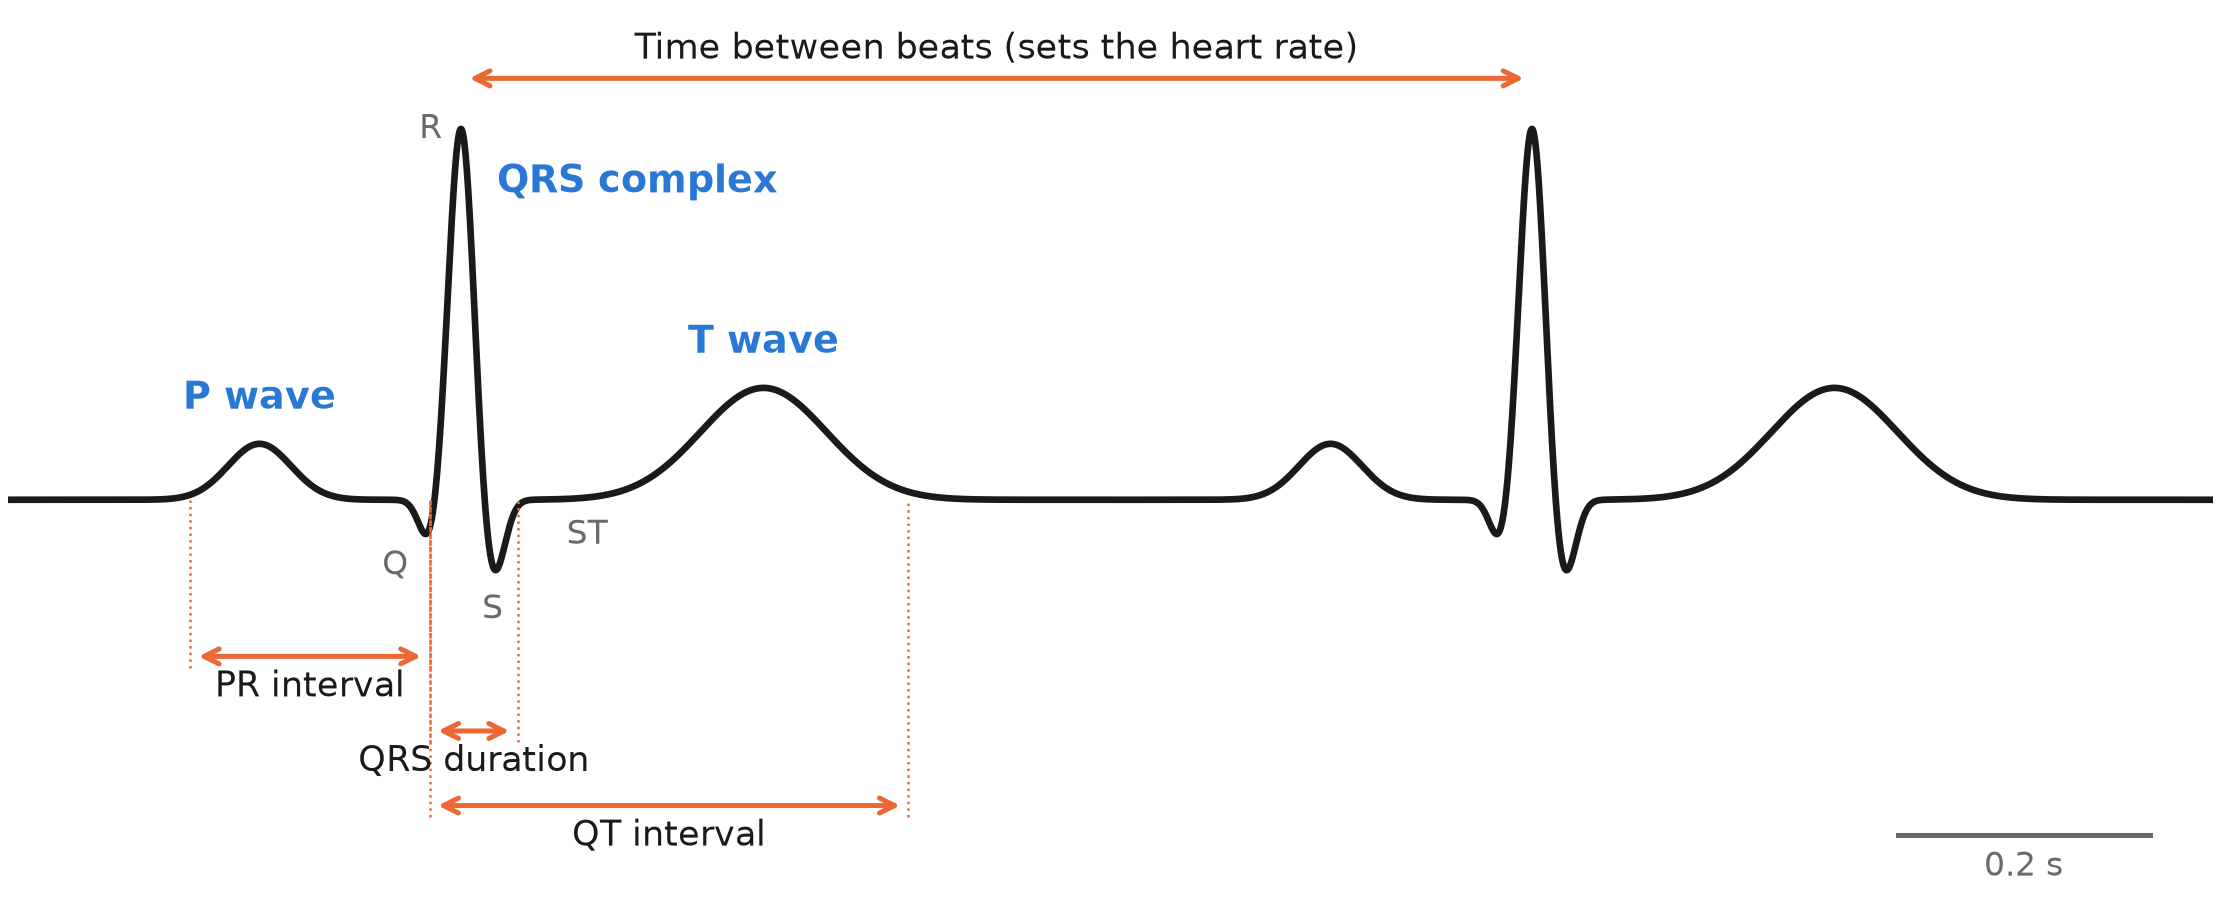
\includegraphics[width=0.78\linewidth]{figuras/fig_ecg_beat.png}
  \caption{Two heartbeats in one lead, drawn schematically. Each beat has a P wave, a QRS complex (the Q, R and S deflections) and a T wave. The orange spans mark the intervals a reader measures; ST is the segment between the QRS complex and the T wave.}
  \label{fig:beat}
\end{figure}

The model's output is a score per ECG and a decision to flag it or not. It can be wrong in two ways, and the two errors do not cost the same. A missed abnormal ECG (false negative) defeats the purpose of the screening, because that student is not called back. A flagged normal ECG (false positive) costs a reading and may worry the student, but the cardiologist corrects it. The model is meant to order the cardiologist's work; it does not diagnose.

\subsection{The approach we finally adopted}

The project was planned around a dataset of student ECGs from a partner university in Italy, expected to contain about 2,000 labeled recordings. That dataset did not become available during the project. We changed the plan in two ways.

First, all development uses public hospital databases whose ECGs were read by physicians. PTB-XL \parencite{wagner2020ptbxl} carried the first four stages, and the final stage adds five more sources so that the model sees more than one hospital. Second, because no student data exist to test on, we replaced the question ``how well does the model work on students?'' with one we can answer: ``how well does a model trained on some hospitals work at a hospital it has never seen?'' We hold out one complete hospital database for this purpose. A good result there is necessary for the student setting but does not establish it, and Section~\ref{sec:conclusions} returns to this gap.

The same constraint shaped two design choices that recur below. The expected size of the local dataset, about 2,000 labels, led us to prefer methods that work with few labels, including encoders pretrained without labels on millions of ECGs. And since the fraction of abnormal ECGs in students is unknown and certainly far below the hospital figure, we never fix a decision threshold on hospital data: the threshold is set from normal ECGs of the place where the model runs.

\subsection{Objective and acceptance criteria}

The objective is a model that, for a fixed share of normal ECGs sent to review, recovers as many abnormal ECGs as possible. There is no previous automatic system for this population to compare against. We therefore fixed our acceptance criteria before training each stage, using three references: chance, a rule that needs no learning, and the published benchmark on the same data \parencite{strodthoff2021deep}. The criteria, and the results against them, are collected in Table~\ref{tab:criteria} in Section~\ref{sec:results}.

One criterion is missing on purpose. We did not set a minimum sensitivity for clinical use, because that number depends on what the service can absorb and on which findings matter in young people. Both are clinical decisions, and validation with a cardiologist is still pending.

% =====================================================================
\section{Data and preparation}
% =====================================================================

\subsection{PTB-XL and the label}
\label{sec:label}

PTB-XL version 1.0.3 contains 21,799 ten-second, 12-lead ECGs from 18,869 patients, sampled at 500~Hz \parencite{wagner2020ptbxl}. Each recording has a coded report, and the codes are grouped into five superclasses: normal (NORM), myocardial infarction (MI), ST-T changes (STTC), conduction disturbance (CD) and hypertrophy (HYP). In plain terms, MI codes mark traces of a past or ongoing heart attack, such as deep Q waves; STTC codes mark a displaced ST segment or an inverted T wave; CD codes mark slow conduction, such as a wide QRS complex or a long PR interval; and HYP codes mark the unusually tall QRS voltages of an enlarged chamber.

The screening question is binary, so we define one label for the whole project. An ECG is positive if it carries at least one MI, STTC, CD or HYP code, and negative if NORM is its only diagnostic code. The 411 ECGs without any diagnostic code are left out, as is one recording with a flat lead, which leaves 21,387 ECGs. We fixed this definition before looking at any model result.

This label is a proxy, and the rest of the article depends on reading it correctly. It records what a physician wrote about the tracing. It is not a confirmed diagnosis, it groups findings with very different consequences, and it leaves out rhythm disorders. In the training folds, 33\% of the labels were not validated by a human, against none in the validation and test folds. We use the word ``abnormal'' below only in this sense.

We use the ten folds published with the dataset, which keep all ECGs of a patient in one fold. Folds 1--8 are for training (17,083 ECGs, 14,822 patients), fold 9 for validation (2,146 ECGs) and fold 10 for testing (2,158 ECGs). About 58\% of the ECGs are positive in each partition, which reflects a hospital population and is far from what a student population would show.

\subsection{From waveform to measurements}

Our first representation follows what a human reader measures. We filter each signal with a zero-phase Butterworth band-pass filter (0.5--40~Hz), detect the beats, average them into one median beat per lead, and locate the P wave, the QRS complex and the T wave on it. From these we take 132 primary measurements (amplitudes, durations, intervals, rhythm statistics) and 22 derived indices that clinicians use, such as the heart-rate-corrected QT interval and voltage sums for hypertrophy. Skewed variables are power-transformed and all continuous variables are standardized, with every parameter fitted on the training folds only.

Before trusting the measurements, we checked them against codes they should explain: the measured QRS duration separates ECGs annotated with a complete bundle branch block (a wide QRS) from normal ones with an AUROC of 0.99. We then removed columns that carried no information or duplicated another one, with variance, relevance and correlation filters, which reduced the encoded matrix from 163 to 111 columns.

The decisive step of this stage was building the measurements, not selecting among them. A logistic regression on 24 generic signal summaries reached a validation AUROC of 0.801; on the constructed measurements it reached 0.930, and no later filtering or projection step moved that figure by more than 0.03. The 111 selected columns gave 0.929 with a third fewer inputs.

We also decided what the model must not see. In PTB-XL, age alone predicts the label with an AUROC of 0.771 and the recording device alone with 0.657, because of how the database was assembled. Age, sex, device, site and every field written by the reader are therefore excluded from the inputs.

\subsection{A multi-source training cohort and an external hospital}
\label{sec:cohort}

A model fitted on one hospital can learn that hospital's devices and habits, and cross-validation inside a single source then overstates how it will do elsewhere \parencite{leinonen2024empirical}. For the final stage we therefore assembled a training cohort of 25,000 ECGs from six public sources, all obtained from PhysioNet \parencite{goldberger2000physiobank}: Ningbo (9,952 ECGs) and Chapman-Shaoxing (3,050) \parencite{zheng2022ningbo,zheng2020database}, PTB-XL (6,828), and three sets released with the 2020 PhysioNet/Computing in Cardiology Challenge \parencite{perezalday2020classification}, Georgia (3,974) and two from the China Physiological Signal Challenge (1,196) \parencite{liu2018open}. In total 17,607 ECGs are abnormal and 7,393 normal. A source qualifies only if its labels come from human readers, which rules out two much larger collections, MIMIC-IV-ECG and CODE-15\%, whose labels we treat as machine-generated. A record enters if it lasts ten seconds, passes a signal-quality check, has a defined label and matches no evaluation record; from PTB-XL we take only folds 1--7. Appendix~\ref{app:cohort} gives the composition by source (Table~\ref{tab:cohort}) and the complete rules, which we fixed before selecting any record.


For this cohort we use 130 raw waveform measurements without the PTB-XL-specific selection step, and fit imputation and scaling inside each training fold.

A cohort of several hospitals still cannot tell us how the model behaves at a hospital that contributed nothing to it, and that is the situation of any new screening site. We therefore keep one complete database out of training: the Shandong Provincial Hospital (SPH) database \parencite{liu2022large}. It was recorded at a different hospital, with other devices, and annotated by another team under a different coding scheme than any training source. This follows the practice of the benchmarks from which we later take our pretrained encoders, which score each model on datasets held out from its training \parencite{almasud2025benchmarking,lunelli2026benchecg}; a score on held-out folds of the training sources would not separate what the model learned about ECGs from what it learned about those sources. No SPH recording enters training or hyperparameter selection, and SPH is not among the pretraining sources reported for the encoder we use. We split its ECGs once into 6,968 normal ECGs used only to set the threshold (the calibration normals) and 10,434 ECGs used only for evaluation, of which 3,584 are abnormal (34.3\%). Fold 9 of PTB-XL is the second evaluation set. Fold 10 of PTB-XL and the reserved groups of the Challenge sources were not scored in the final stage.

Two limitations of these data carry through to the results. The Challenge sources do not publish patient identifiers, so their folds are split by record and we cannot rule out that one patient contributes ECGs to two folds. And the population is far from the target: the median age in PTB-XL is 62 years and only 6.3\% of its ECGs come from people under 30. This matters for specific measurements. Among normal PTB-XL ECGs of men under 30, 95.1\% show an ST elevation of at least 0.1~mV in lead V2, a pattern that is common in healthy young men and would count as suspicious in an older patient. Parameters fitted on hospital patients cannot be carried over to students without checking this difference.

% =====================================================================
\section{Methodology and models}
% =====================================================================

The modelling went through three stages: a baseline, a search among single models, and a final model that combines two views of the signal. All three share one evaluation protocol, which we describe first because it decides how every later number should be read.

\subsection{Metrics and the referral budget}
\label{sec:budget}

Accuracy is the wrong metric for this problem. If 2\% of students had an abnormal ECG, a model that calls everyone normal would be 98\% accurate and find no one. We need metrics that do not change with the fraction of positives. The AUROC is the probability that a randomly chosen abnormal ECG receives a higher score than a randomly chosen normal one, so it depends only on how the model orders ECGs. We use it to compare models and to choose hyperparameters. We also report average precision, the area under the precision-recall curve, but do not decide with it because precision changes with prevalence.

A ranking is not yet a decision: the service needs a threshold. A fixed cut such as 0.5 fails because the scores are not calibrated probabilities, and a threshold tuned for a target sensitivity needs abnormal cases, which a student service has few of. In the baseline stage, a threshold set on training normals transferred well to the test fold (90.7\% specificity for a 90\% target), while one set on abnormal ECGs for 95\% sensitivity reached only 91.5\%.

We therefore define the operating point from normal ECGs alone. The service states how many normal ECGs it accepts to review, the \emph{referral budget} $b$, and the threshold is the score that only a fraction $b$ of local normal ECGs exceed. Formally, if $s_1,\dots,s_m$ are the scores of $m$ calibration normals,
\begin{equation}
  t_b = \text{the smallest } t \text{ such that } \frac{1}{m}\sum_{i=1}^{m} \mathbf{1}[s_i > t] \le b ,
  \label{eq:budget}
\end{equation}
and a new ECG with score $s$ is flagged when $s > t_b$. With $b = 0.05$ and 6,968 calibration normals, at most 348 of them lie above the threshold. The budget bounds the false alerts, not the total referrals: abnormal ECGs that the model detects are referred on top of it. Sensitivity at a given budget is the quantity we want to raise. Normal ECGs are also the easiest recordings to collect in a student population.

Confidence intervals come from 2,000 bootstrap resamples of whole patients, because some patients have several ECGs.

\subsection{Baseline: a linear model on measurements}

The baseline has to be simple enough to explain and strong enough to be worth beating. Below it we placed a reference with no learning at all: count how many of eight textbook criteria an ECG meets (for example a QRS of 110~ms or longer, an inverted T wave, a heart rate outside 60--100 beats per minute). This rule reaches an AUROC of 0.785 on the training folds, which shows the problem is tractable, but 15.0\% of the abnormal ECGs meet none of the criteria, so the rule cannot reach high sensitivity without flagging everyone.

For the baseline we chose an L2-regularized logistic regression on the 111 measurements: the inputs are tabular and standardized, there are about 150 training ECGs per parameter, and the coefficients can be read directly. Eight-fold cross-validation with the one-standard-error rule gave $C = 0.1$. The model does not overfit (training AUROC 0.939, cross-validated 0.935), and its learning curve is flat beyond 9,000 ECGs. It underfits slightly, since gradient boosting on the same inputs reaches 0.955. Shuffling groups of features shows what it relies on: the AUROC falls by 0.199 without the ST-T measurements and by 0.129 without the QRS measurements.

\subsection{Single-model candidates}

The baseline's mild underfitting suggests that a non-linear decision boundary would help. We compared seven algorithms of different families on the same folds, all as implemented in scikit-learn \parencite{pedregosa2011scikitlearn}: logistic regression, linear discriminant analysis, Gaussian naive Bayes, $k$-nearest neighbours, a decision tree, a support vector machine (SVM) with a radial basis function kernel, and a multilayer perceptron (MLP). Only the last two beat the baseline (Table~\ref{tab:single}). A quick search over the main hyperparameter of the four weaker models (53 configurations) left all of them below the baseline, so the ranking does not depend on default settings.

\begin{table}[H]
  \centering
  \caption{Single models on PTB-XL with 111 measurements. CV: mean AUROC over eight training folds (standard deviation between folds 0.004 to 0.013). Fold 10 was scored once per stage, after all choices; brackets are 95\% patient-bootstrap intervals. Gradient boosting is an ensemble, shown only as a reference.}
  \label{tab:single}
  \begin{tabular}{lccc}
    \toprule
    Model & AUROC, CV & AUROC, fold 9 & AUROC, test fold 10 \\
    \midrule
    Criteria count (no learning)   & 0.785  & 0.782  & 0.760 [0.740, 0.780] \\
    Decision tree                  & 0.813 & 0.808 & -- \\
    $k$-nearest neighbours         & 0.899 & 0.890 & -- \\
    Gaussian naive Bayes           & 0.915 & 0.915 & -- \\
    Linear discriminant analysis   & 0.924 & 0.918 & -- \\
    Logistic regression (baseline) & 0.935 & 0.928 & 0.917 [0.905, 0.929] \\
    MLP, tuned                     & 0.949 & 0.940 & 0.933 [0.922, 0.943] \\
    SVM, tuned                     & 0.951 & 0.939 & 0.933 [0.923, 0.944] \\
    \midrule
    Gradient boosting (reference)  & 0.955 & 0.943 & 0.937 [0.927, 0.947] \\
    \bottomrule
  \end{tabular}
\end{table}

We then tuned the two leaders with 146 configurations and 1,168 model fits (Appendix~\ref{app:search}). Both searches ended on plateaus: the tuned SVM ($C = 3$, $\gamma = 0.0056$) gained 0.0002 over its default configuration and the tuned MLP (one hidden layer of 128 ReLU units) gained 0.0006.

The two tuned models cannot be told apart by AUROC: on the test fold the difference is $+0.0009$ $[-0.0022, +0.0041]$. We chose on other grounds. Trained on about 1,500 ECGs, close to the size expected for the local dataset, the SVM kept an AUROC of 0.936 while the MLP fell to 0.923, the level of the baseline. The SVM is also deterministic; the MLP is cheaper to run. We selected the SVM and carried both models into the next stage.

\subsection{A second view of the signal: pretrained encoders}

Every model so far sees the ECG through measurements that we designed. Anything the measurements miss, such as a subtle change of wave shape, is invisible to them. The alternative is to let a network learn its own features from the raw signal, but training such a network from scratch needs far more labels than this project will have.

Self-supervised pretraining addresses exactly this. An encoder is first trained on a large collection of unlabeled ECGs to solve a task built from the signal itself, and its internal representation is then reused for a labeled task. We considered three published encoders, which differ in the pretraining task:

\begin{itemize}\setlength{\itemsep}{0pt}\setlength{\parskip}{0pt}
  \item ECG-CPC applies contrastive predictive coding \parencite{vandenoord2018cpc} to ECGs: the model summarizes the signal up to a time point and must pick the true representation of the next segment among distractors. We use the released model with a structured state space (S4) backbone evaluated by \textcite{almasud2025benchmarking}.
  \item ECG-JEPA \parencite{kim2024ecgjepa} follows the joint-embedding predictive architecture \parencite{assran2023ijepa}: parts of the ECG are hidden and the model predicts their representations, not their samples, from the visible parts. Predicting in representation space avoids spending capacity on noise.
  \item xECG \parencite{lunelli2026benchecg} is an encoder built from extended long short-term memory (xLSTM) blocks \parencite{beck2024xlstm}, a recurrent architecture whose cost grows linearly with signal length. It has 57 million parameters and was pretrained on about 8.2 million recordings.
\end{itemize}

We use these encoders frozen: the ECG goes through the published weights unchanged, the pooled output vector is the feature, and only a logistic regression on top of it is trained. This is the linear-probing protocol of the benchmarks that evaluate ECG foundation models \parencite{almasud2025benchmarking,lunelli2026benchecg}. It suits our case for three reasons. A linear head has few parameters, so it can be fitted with a few thousand labels. The expensive encoder pass is done once per ECG and cached. And a frozen encoder cannot adapt to the quirks of the training hospitals.

To choose one encoder we gave all three the same task: fit a logistic head ($C = 0.01$) on PTB-XL folds 1--7, set the threshold on the normal ECGs of fold 8 and evaluate on fold 9. Table~\ref{tab:encoders} shows the result. xECG and ECG-JEPA are close, and both are clearly ahead of ECG-CPC. We continued with xECG. The comparison is between published checkpoints with different pretraining data and budgets, so it tells us which checkpoint serves this task and says nothing general about the three architectures. We also checked the pretraining sources reported by the xECG authors: they include neither PTB-XL nor SPH, so both evaluation sets are new to the encoder.

\begin{table}[H]
  \centering
  \caption{Three published self-supervised encoders, frozen, with the same logistic head on PTB-XL (fit on folds 1--7, threshold from fold 8 normals at a 5\% budget, evaluation on fold 9).}
  \label{tab:encoders}
  \begin{tabular}{lccccc}
    \toprule
    Encoder & Feature size & AUROC & Avg.\ precision & Sensitivity & Specificity \\
    \midrule
    xECG       & 1,024 & 0.943 & 0.961 & 0.740 & 0.963 \\
    ECG-JEPA   &   768 & 0.941 & 0.959 & 0.739 & 0.954 \\
    ECG-CPC (S4) & 512 & 0.919 & 0.945 & 0.687 & 0.962 \\
    \bottomrule
  \end{tabular}
\end{table}

\subsection{The final model: averaging two views}

The measurements describe defined properties of the waveform; the encoder contributes features learned from millions of ECGs. If the two views make different mistakes, combining them should beat either one. The final stage tests this, together with more conventional ensembles, on the 25,000-ECG cohort of Section~\ref{sec:cohort}.

We compared nine recipes. Four are single models: logistic regression, the SVM and the MLP on the 130 measurements, and the frozen xECG encoder with a logistic head. Five are ensembles: a random forest of 160 trees and histogram-based gradient boosting (both homogeneous), voting and stacking of the SVM and the MLP, and a \emph{blend} that averages the boosting score and the xECG score with equal weights,
\begin{equation}
  s_{\text{blend}}(x) = \tfrac{1}{2}\, p_{\text{boost}}\big(m(x)\big) + \tfrac{1}{2}\, p_{\text{xECG}}\big(e(x)\big),
\end{equation}
where $m(x)$ are the 130 measurements of ECG $x$ and $e(x)$ is its 1,024-dimensional xECG representation. The weights are fixed at one half and are not fitted, which leaves nothing to overfit in the combination step. Figure~\ref{fig:pipeline} shows the complete path from signal to decision.

\begin{figure}[H]
  \centering
  \resizebox{\linewidth}{!}{%
  \begin{tikzpicture}
    \node[box, text width=1.9cm] (ecg) at (0,0) {12-lead ECG\\10 s, 500 Hz};
    \node[box, text width=1.9cm] (qc) at (2.9,0) {Signal-quality check};
    \node[box, text width=2.5cm] (meas) at (6.2,0.85) {130 waveform measurements};
    \node[box, text width=2.5cm] (enc) at (6.2,-0.85) {Frozen xECG encoder};
    \node[box, text width=1.9cm] (hgb) at (9.5,0.85) {Gradient boosting};
    \node[box, text width=1.9cm] (lr) at (9.5,-0.85) {Logistic head};
    \node[box, text width=1.5cm] (avg) at (12.2,0) {Average of the two scores};
    \node[box, text width=1.5cm] (thr) at (14.6,0) {Flag if score $> t_b$};
    \node[box, text width=2.3cm, fill=white] (cal) at (14.2,-2.0) {Local normal ECGs set $t_b$};
    \node[box, text width=2.6cm, fill=white] (abst) at (2.9,-2.0) {Abstain: repeat or read directly};
    \draw[flow] (ecg) -- (qc);
    \draw[flow] (qc.east) -- ++(0.35,0) |- (meas.west);
    \draw[flow] (qc.east) -- ++(0.35,0) |- (enc.west);
    \draw[flow] (meas) -- (hgb);
    \draw[flow] (enc) -- (lr);
    \draw[flow] (hgb.east) -- ++(0.35,0) |- ([yshift=2mm]avg.west);
    \draw[flow] (lr.east) -- ++(0.35,0) |- ([yshift=-2mm]avg.west);
    \draw[flow] (avg) -- (thr);
    \draw[side] (cal.north -| thr) -- (thr);
    \draw[side] (qc) -- node[right, role] {fails} (abst);
  \end{tikzpicture}}
  \caption{The final model. Each ECG that passes the quality check is described twice, by waveform measurements and by a pretrained encoder; each description feeds its own classifier and the two scores are averaged. The threshold $t_b$ comes from normal ECGs of the site where the model runs (Equation~\ref{eq:budget}). Dashed arrows are side paths.}
  \label{fig:pipeline}
\end{figure}

Hyperparameters were chosen with three grouped folds inside the training cohort, keeping known patients together. After the plateaus of the previous stage the search was small (Appendix~\ref{app:search}): boosting trees with 31 leaves and a learning rate of 0.08, and $C = 0.1$ for the xECG head.

We fixed the selection rule before scoring either evaluation hospital: choose the recipe with the highest out-of-fold AUROC on the training cohort. The blend reached 0.980, against 0.977 for boosting alone and 0.977 for xECG alone, and was selected. Only then did we compute the hospital results of Section~\ref{sec:results}, which describe the chosen model and played no part in choosing it.

One further experiment tested whether the frozen encoder leaves performance unused. We fine-tuned all xECG parameters with the head for one pass over the 25,000 ECGs (9.8 minutes on a graphics card). The adoption rule, fixed in advance, asked for at least two more points of sensitivity on SPH with an interval above zero and at most half a point more false positives.

% =====================================================================
\section{Results and validation}
\label{sec:results}
% =====================================================================

\subsection{Performance at the external hospital}

Table~\ref{tab:final} gives the nine recipes at both evaluation sites, each with its own threshold from that site's calibration normals at a 5\% budget. On SPH the selected blend has the highest AUROC (0.937) and the highest sensitivity (77.4\%). Its two components come next, and the ensembles that combine two models of the same view (voting and stacking of SVM and MLP) gain almost nothing over their members.

\begin{table}[!htb]
  \centering
  \caption{Final-stage comparison. All recipes are fitted on the same 25,000 ECGs. SPH: 10,434 evaluation ECGs from the external hospital; sensitivity and specificity at a threshold that flags 5\% of that hospital's calibration normals. Fit time is the final fit on cached features, in seconds, and excludes feature extraction.}
  \label{tab:final}
  \begin{tabular}{lccccc}
    \toprule
     & \multicolumn{3}{c}{SPH (external)} & PTB-XL fold 9 & \\
    \cmidrule(lr){2-4}\cmidrule(lr){5-5}
    Recipe & AUROC & Sens. & Spec. & AUROC & Fit (s) \\
    \midrule
    \textbf{Blend: boosting + xECG} & \textbf{0.937} & \textbf{0.774} & 0.951 & \textbf{0.926} & 3.7 \\
    Frozen xECG + logistic head   & 0.932 & 0.761 & 0.950 & 0.920 & 2.1 \\
    Histogram gradient boosting   & 0.927 & 0.747 & 0.945 & 0.919 & 1.6 \\
    Random forest                 & 0.925 & 0.726 & 0.950 & 0.915 & 27.9 \\
    Stacking, SVM + MLP           & 0.914 & 0.708 & 0.947 & 0.918 & 38.5 \\
    Voting, SVM + MLP             & 0.914 & 0.708 & 0.948 & 0.918 & 15.1 \\
    SVM on measurements           & 0.913 & 0.702 & 0.948 & 0.918 & 6.4 \\
    MLP on measurements           & 0.913 & 0.703 & 0.949 & 0.918 & 8.7 \\
    Logistic regression on measurements & 0.883 & 0.599 & 0.957 & 0.893 & 0.3 \\
    \bottomrule
  \end{tabular}
\end{table}

The gain of the blend over its stronger component is small but measurable. The AUROC difference between the blend and xECG alone on SPH is $+0.0052$, with a 95\% interval of $[0.0034, 0.0072]$. This interval reflects resampling of patients for fixed models; it does not include the variation from retraining or from moving to another hospital. Figure~\ref{fig:roc}a shows that the three curves separate only at the left edge, where few normal ECGs are flagged. That is the region in which the model operates.

\begin{figure}[!htb]
  \centering
  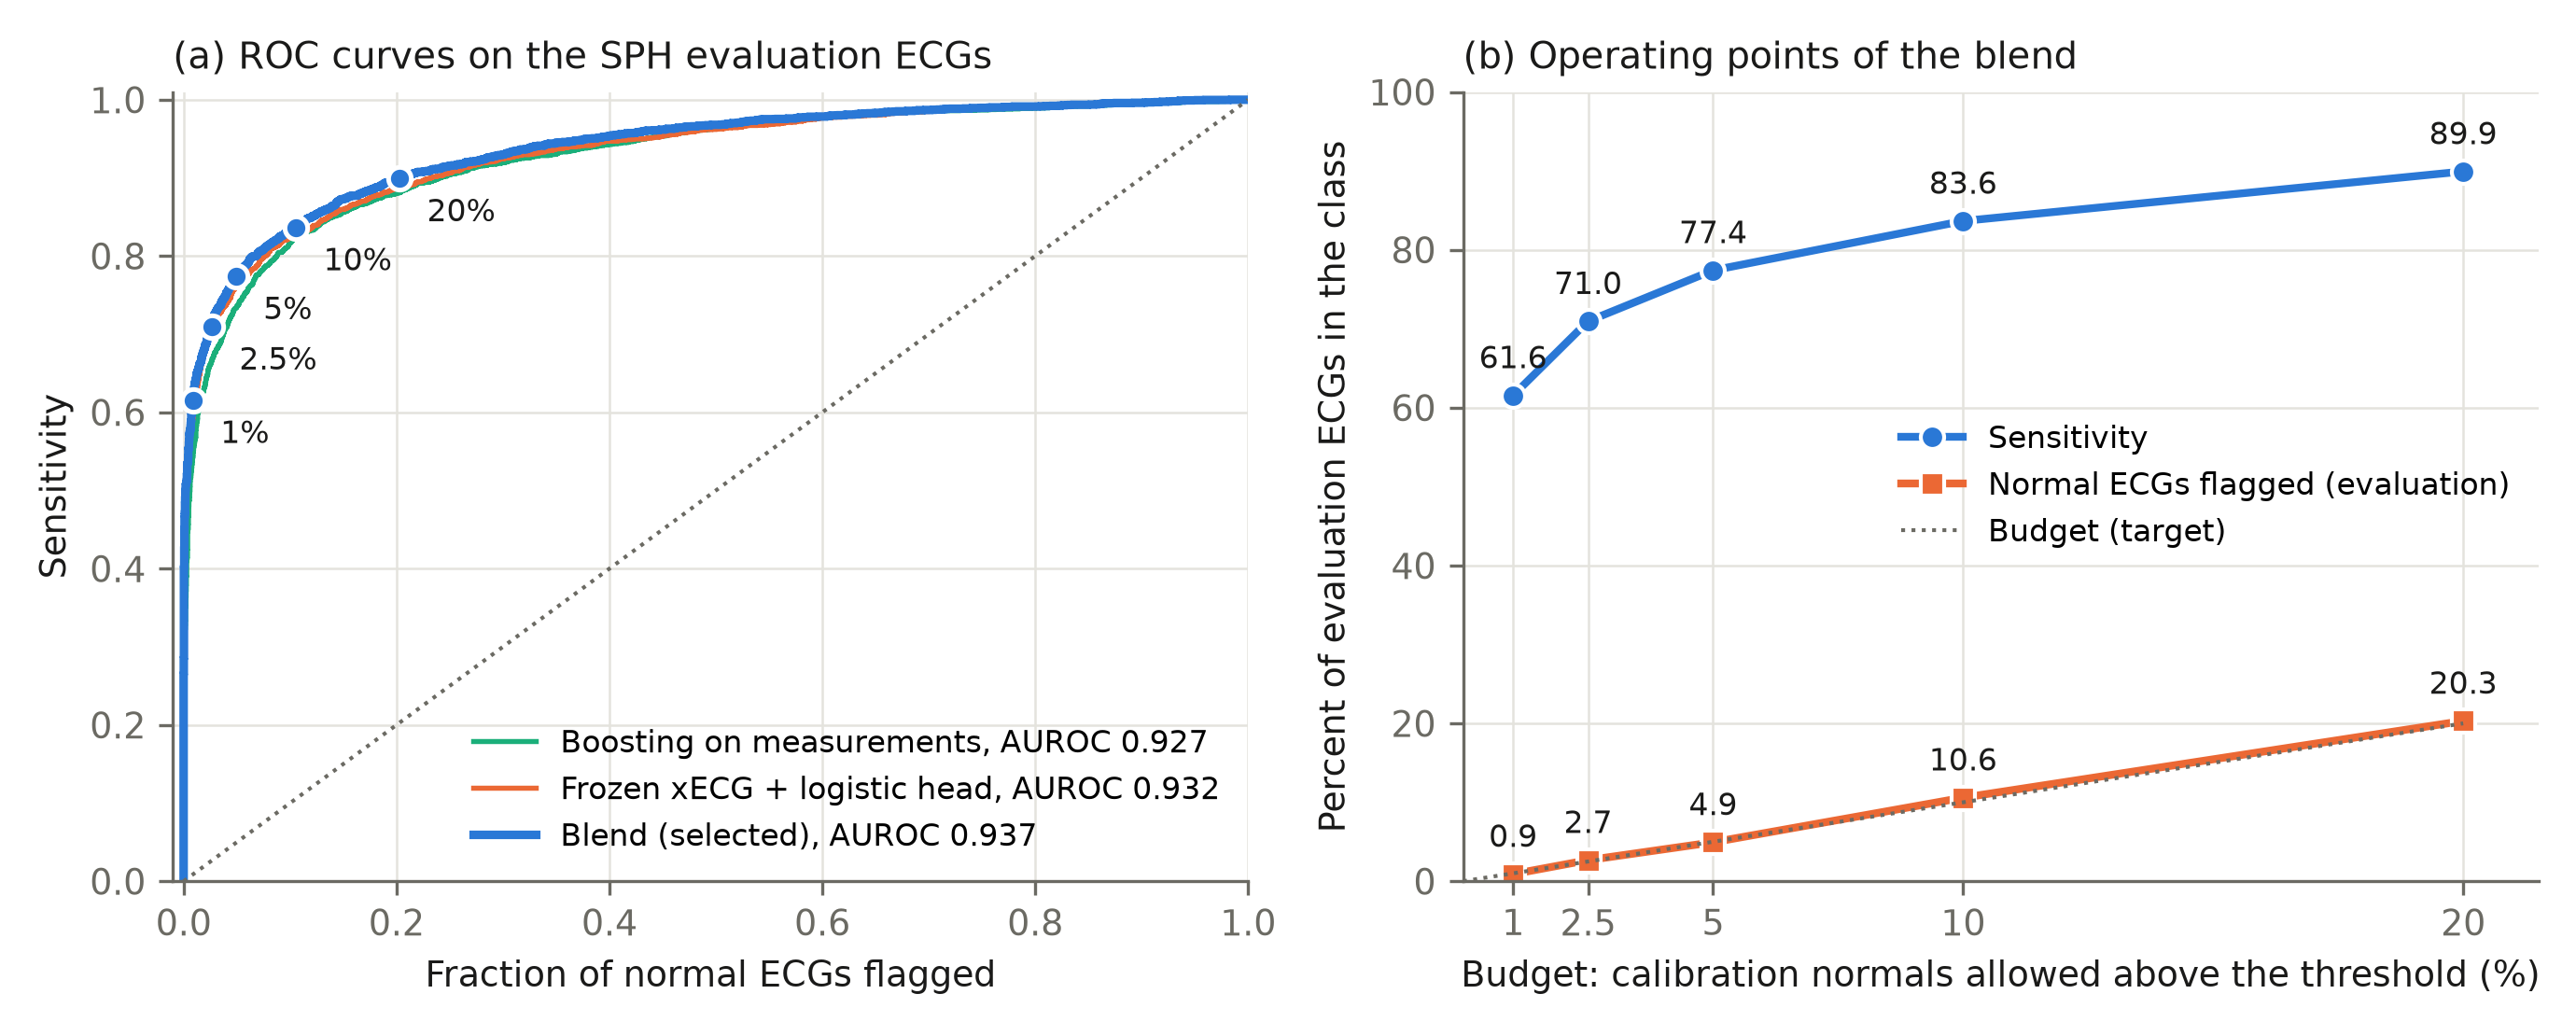
\includegraphics[width=0.88\linewidth]{figuras/fig_roc_budget.png}
  \caption{The selected model on the 10,434 SPH evaluation ECGs. (a) ROC curves of the blend and its two components; the points mark the blend's operating points for five referral budgets. (b) For each budget, the sensitivity reached and the percentage of evaluation normals actually flagged. The flagged percentage follows the budget closely; sensitivity grows more and more slowly.}
  \label{fig:roc}
\end{figure}

\subsection{What the errors mean for the service}

At the 5\% reference budget the threshold is 0.680, and the 10,434 evaluation ECGs divide as follows. Of 3,584 abnormal ECGs, the model flags 2,774 and misses 810. Of 6,850 normal ECGs, it flags 338 (4.9\%, against a target of 5\%) and passes 6,512. The cardiologist would open 3,112 ECGs, 29.8\% of the total, and 89.1\% of them would be abnormal.

The 810 misses are the main limitation. They are 22.6\% of the abnormal ECGs and more than twice the number of false alerts. This follows from choosing a budget that keeps the reading load low, and it means that at this budget the model cannot be the only filter: ECGs below the threshold are unflagged, not cleared. A service that cannot accept this many misses has to accept a larger budget, and Figure~\ref{fig:roc}b and Table~\ref{tab:budgets} (Appendix~\ref{app:budgets}) price that choice. Moving from a 1\% to a 2.5\% budget recovers 337 more abnormal ECGs for 121 more false alerts, about one false alert for every three additional detections. From 5\% to 10\% the ratio is 1.7 false alerts per additional detection, and from 10\% to 20\% it is 3.0. The 5\% budget is the last step at which one more detection costs less than one unnecessary reading. The right budget remains the service's decision.

Counts show what the blend buys at the same budget. Against xECG alone it detects 47 more abnormal ECGs with 2 fewer false alerts; against boosting alone, 96 more with 40 fewer. Logistic regression on measurements produces only 292 false alerts but detects 2,146 abnormal ECGs: it would save 46 readings and lose 628 detections.

The precision of 89.1\% must not be carried over to students. Precision depends on how common abnormal ECGs are, and at SPH they are 34.3\% of the evaluation set. Two studies of young athletes in the United States found relevant cardiovascular conditions in 13 of 5,258 college athletes \parencite{drezner2016electrocardiographic} and 16 of 3,620 high-school athletes \parencite{williams2019performance}, that is, 0.2\% to 0.4\%. If the sensitivity and specificity measured at SPH held at such a prevalence, 10,000 screened people would produce about 490 false alerts and 19 to 34 true detections: between 4 and 7 of every 100 alerts would be true (Appendix~\ref{app:projection}). This is arithmetic under a strong assumption, since our sensitivity is measured against ECG annotations and those studies count clinical conditions. The order of magnitude is what matters: in a student population most alerts will be false at any budget.

\subsection{An optional aid: which part of the tracing drives the score}
\label{sec:where}

A score tells the cardiologist which ECG to open. It does not say where to look in it. Alongside the classifier we built a display for that narrower question: which lead, and which wave, does the score depend on?

The method is an occlusion test with a meaningful replacement. For one ECG, we replace one wave (P, QRS or ST-T) in one lead with the wave expected in a normal ECG of the same heart rate, age and sex, recompute both feature sets and the blend, and record how far the score falls. Twelve leads and three waves give a $12 \times 3$ map. A large fall means the model relied on that region.

Figure~\ref{fig:where} shows the map for one SPH recording annotated as an infarction. Its score is 0.992. The largest falls are in the QRS complex of leads V5 and II (0.006 each) and in the ST-T segment of aVR (0.004) and no single region comes close to removing the alert. Replacing the QRS complex in all twelve leads lowers the score by 0.098, and replacing the whole ECG by 0.417, which takes it below the threshold. The alert rests on information spread over several leads.

\begin{figure}[!htb]
  \centering
  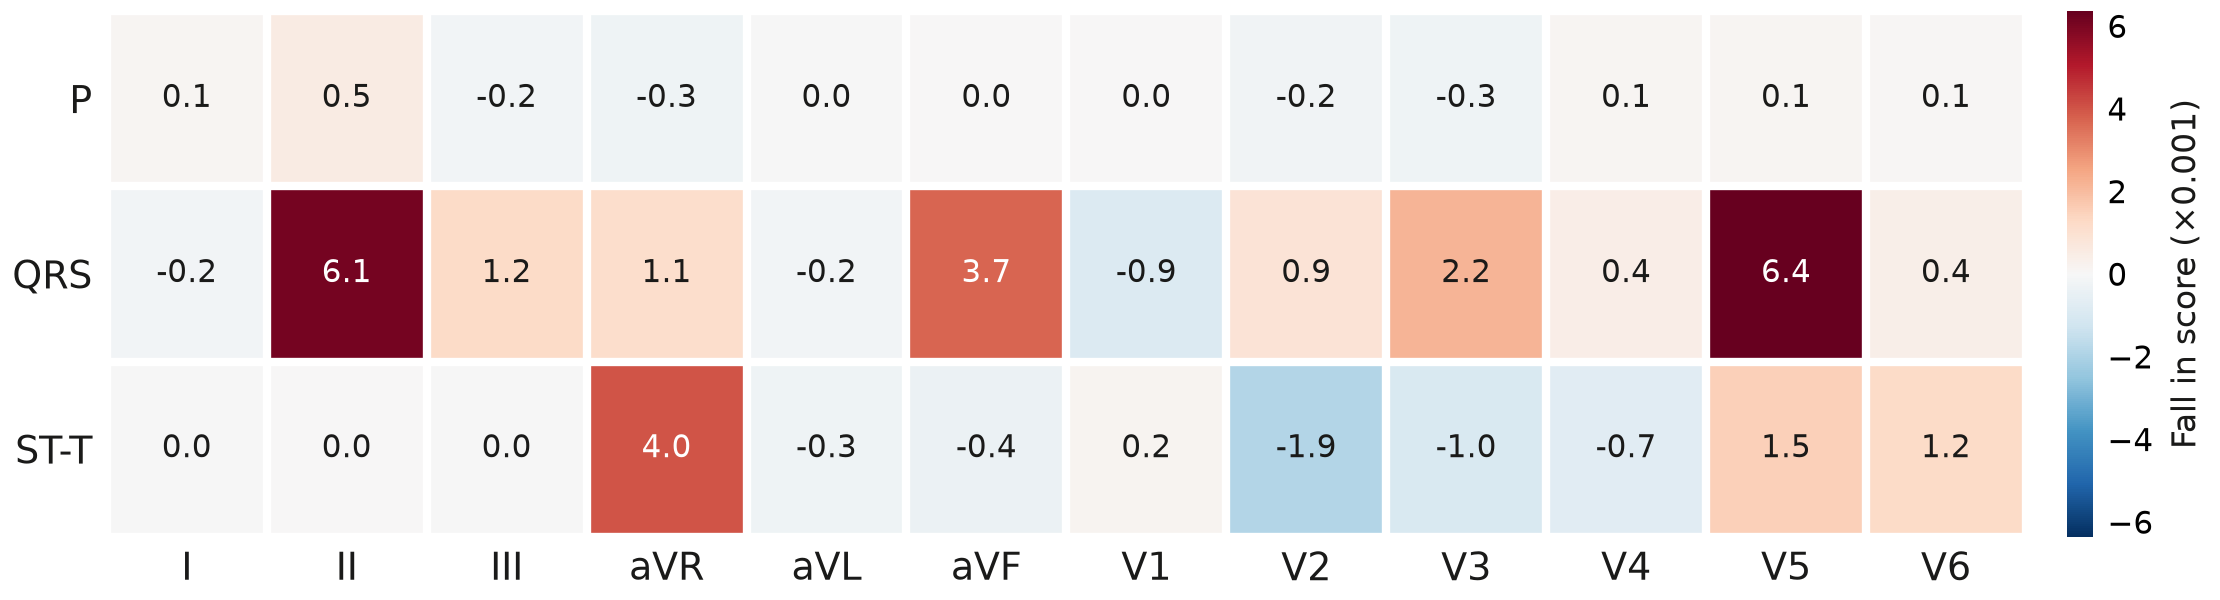
\includegraphics[width=0.8\linewidth]{figuras/fig_where.png}
  \caption{Fall in the blend score, in thousandths, when one wave of one lead is replaced by its normal counterpart, for one SPH recording annotated as an infarction (original score 0.992). Red: the region supported the alert. Blue: replacing it raised the score.}
  \label{fig:where}
\end{figure}

Whether the map points to the right place depends on how closely one looks. Averaged over ECGs of one type it does: for ECGs annotated with a right bundle branch block (a wide QRS complex of a typical shape) the QRS complex carries 79\% of the attribution, and for ECGs annotated with ST-T changes the ST-T segment carries 85\%. Lead by lead it does not. In 104 infarction ECGs, the lead with the largest fall lay in the region named by the annotation in 49.0\% of cases, while a control that uses only the energy of the replaced signal reached 56.7\%.

We therefore present the map as an aid under development (details in Appendix~\ref{app:where}). It shows what drives the model's score, which is not the same as where a lesion is. In the prototype it is a separate view that the cardiologist can leave switched off, and the flag never depends on it.

\subsection{Results against the criteria fixed in advance}

Table~\ref{tab:criteria} sets each criterion beside what we observed. The baseline met its three conditions. The fine-tuned encoder detected 43 fewer abnormal ECGs and raised 20 more false alerts than the frozen one, so it was rejected. Against the baseline, the best single model added 0.016 AUROC on the PTB-XL test fold, and at the external hospital the blend detects 628 more abnormal ECGs than logistic regression fitted on the same cohort, at 46 more false alerts.

\begin{table}[!htb]
  \centering
  \caption{Criteria fixed before each stage, the observed result and the remaining gap. Brackets are 95\% patient-bootstrap intervals. Macro AUROC is the mean over the five PTB-XL superclasses on fold 10, as in the benchmark of \textcite{strodthoff2021deep}.}
  \label{tab:criteria}
  \small
  \begin{tabular}{p{5.6cm}p{5.6cm}p{4.0cm}}
    \toprule
    Criterion & Observed & Outcome \\
    \midrule
    Baseline AUROC above the criteria count, interval excluding zero & $+0.157$ [0.139, 0.175] on fold 10 (0.917 against 0.760) & Met \\
    At 95\% sensitivity, baseline spares more normals than the criteria count & 53.6\% [43.8, 59.1] against 0\% & Met \\
    Macro AUROC of at least 0.874 (feature-based method of the benchmark) & Baseline 0.898 [0.889, 0.907]; SVM 0.919 [0.911, 0.926] & Met; benchmark networks reach 0.921--0.930 \\
    Final recipe: highest out-of-fold AUROC in training & Blend 0.980; boosting 0.977; xECG 0.977 & Blend selected \\
    False alerts within the 5\% budget at the external hospital & 4.9\% of 6,850 normals flagged & Met \\
    Fine-tuning adopted only if sensitivity rises by 2 points or more & $-1.20$ points [$-1.84$, $-0.59$] & Not met; rejected \\
    Minimum sensitivity for clinical use & 77.4\% at a 5\% budget; 89.9\% at 20\% & No target set yet \\
    \bottomrule
  \end{tabular}
\end{table}

Three results limit how far these numbers can be taken.

First, training on more hospitals did not improve the PTB-XL score. The PTB-XL-only models reached about 0.94 on fold 9 (Table~\ref{tab:single}); the multi-source blend reaches 0.926. Data, inputs and label mix all changed between the stages, so the difference has no single cause. What the multi-source model adds is evidence at a hospital it never saw.

Second, the blend's out-of-fold AUROC in training (0.980) is far above its value at either evaluation site (0.926 and 0.937). A pooled score over six sources rewards a model for telling sources apart when their share of positives differs (Table~\ref{tab:cohort}), so it overstates what to expect at a new site. We used it only to rank recipes.

Third, no evaluation set is untouched. Fold 10 of PTB-XL was scored at the end of two stages, and fold 9 and SPH were read repeatedly during development. These are development results, not a final test.

We also tried to move the training data towards the target population by preferring ECGs of people aged 18 to 25 (Appendix~\ref{app:age}). Sensitivity on SPH changed by $+0.47$ points $[-0.72, +1.64]$, below the two-point margin fixed in advance, and a 25,000-ECG selection that preferred young people still had a median age of 62. We kept the general cohort.

% =====================================================================
\section{Implementation and operation}
% =====================================================================

The model has been run only on stored public data and in a local prototype. This section proposes the design of a supervised pilot: what it takes to operate the model, who should own each part, and what to watch.

\subsection{Deployment architecture}

A student screening campaign produces a small volume of ECGs, and the recordings are health data. Both facts point to a single machine inside the health service's network, with no ECG leaving the premises. The prototype already runs inference on a processor without a graphics card. A managed cloud service would add elasticity that this workload does not need and would require a data-processing agreement.

Figure~\ref{fig:deploy} shows the proposed components. The nurse exports each recording from the ECG device as twelve leads in millivolts at 500~Hz. The inference service first applies the signal-quality check. If the recording fails, the service abstains and asks for a repeat or a direct reading; an abstention is never reported as a negative. Otherwise it computes the measurements and the encoder features, applies the two frozen classifiers, averages the scores and compares the result with the site's threshold. The cardiologist sees a worklist ordered by score, with the flag and, if switched on, the map of Section~\ref{sec:where}, and records a reading for every ECG opened. Those readings feed two loops: the normal ECGs keep the threshold calibrated, and all readings feed the monitoring report.

\begin{figure}[H]
  \centering
  \resizebox{\linewidth}{!}{%
  \begin{tikzpicture}
    \node[box, text width=2.2cm, minimum height=1.3cm] (dev) at (0,0) {ECG device export};
    \node[box, text width=3.0cm, minimum height=1.3cm] (api) at (4.0,0) {Inference service:\\quality check, features, blend};
    \node[box, text width=2.4cm, minimum height=1.3cm] (list) at (8.0,0) {Worklist ordered by score};
    \node[box, text width=2.2cm, minimum height=1.3cm] (card) at (12.2,0) {Cardiologist's reading};
    \node[box, text width=3.0cm, minimum height=1.3cm, fill=white] (reg) at (4.0,-2.3) {Model registry:\\weights, hashes, threshold};
    \node[box, text width=2.4cm, minimum height=1.3cm, fill=white] (store) at (8.0,-2.3) {Local store:\\scores, readings, logs};
    \node[box, text width=2.2cm, minimum height=1.3cm, fill=white] (mon) at (12.2,-2.3) {Monitoring report};
    \node[role] at (0,1.0) {Nurse};
    \node[role] at (6.0,1.25) {On-premises server, health-service network};
    \node[role] at (12.2,1.0) {Cardiologist};
    \draw[flow] (dev) -- (api);
    \draw[flow] (api) -- (list);
    \draw[flow] (list) -- (card);
    \draw[side] (reg) -- (api);
    \draw[flow] (list) -- (store);
    \draw[flow] (card.south) -- ++(0,-0.35) -| ([xshift=6mm]store.north);
    \draw[flow] (store) -- (mon);
    \draw[side] (mon.south) -- ++(0,-0.4) -| node[pos=0.25, below, role] {recalibrated threshold} (reg.south);
    \node[draw=black!40, dashed, rounded corners=3pt, inner sep=6pt, fit=(api)(list)(reg)(store)] {};
  \end{tikzpicture}}
  \caption{Proposed deployment for a pilot. The components inside the dashed frame run on one server in the health service's network. Solid arrows carry ECGs, scores and readings; dashed arrows carry configuration: the registry supplies the frozen model and the current threshold, and the monitoring loop updates the threshold when the cardiologist's readings of normal ECGs show that it has drifted.}
  \label{fig:deploy}
\end{figure}

The prototype built during the project covers the inference service: a local web application that accepts a recording as a text file of 5,000 rows by twelve leads, runs the quality check before loading any model and abstains on failure. The worklist, the storage of readings and the monitoring report are not built yet.

\subsection{Operating requirements and owners}

Table~\ref{tab:requirements} lists what must be in place before a pilot and who we suggest should answer for it. The most important requirement is the first: the threshold must come from local ECGs that the cardiologist has read as normal. How many are needed depends on the budget. In a resampling experiment on SPH with an earlier xECG-based version of the score, 200 local normals at a 5\% target gave achieved rates between 3.0\% and 7.7\%, and about 1,000 were needed to stay within one point of the target in roughly nine of ten draws.

\begin{table}[!htb]
  \centering
  \caption{Requirements to operate the model in a pilot, with a suggested owner for each.}
  \label{tab:requirements}
  \small
  \begin{tabular}{p{3.2cm}p{8.3cm}p{3.7cm}}
    \toprule
    Requirement & What it involves & Suggested owner \\
    \midrule
    Local calibration set & ECGs from the site's own device, read as normal by the cardiologist; about 1,000 for a 5\% budget; repeated when the device or the population changes & Cardiologist, with the data science team \\
    Referral budget & Share of normal ECGs the service accepts to review, and the rule for ECGs below the threshold during the pilot & Head of the health service and cardiologist \\
    Acquisition standard & Twelve leads in the standard order, millivolts, 500~Hz, ten seconds; repeat the recording when the quality check fails & Nursing staff \\
    Computing & One server in the service's network; a graphics card is optional; end-to-end time per ECG to be measured on that machine & University IT \\
    Model artefacts & Encoder weights, the two classifiers and the threshold, stored with file hashes and a version; no retraining in production & Data science team \\
    Data protection & Informed consent, access control, no recordings or readings outside the service; only aggregate figures in reports & Head of the health service, IT, ethics committee \\
    Clinical definition & Which findings count as positive in young people; the current label is an annotation proxy & Cardiologist \\
    Review and audit & Reading of every flagged ECG and of a random sample of unflagged ones & Cardiologist \\
    Maintenance & Monitoring report, recalibration, response to incidents & Data science team \\
    \bottomrule
  \end{tabular}
\end{table}

Two requirements have no measured value yet: the time of the complete path from recording to score, which includes both feature extractors, and the storage and consent arrangements, which depend on the institution.

\subsection{Monitoring}

A deployed model fails quietly: the scores keep arriving while their meaning changes. Table~\ref{tab:monitoring} lists the signals we would track, chosen so that each known weakness of the model has an observable symptom. The audit of unflagged ECGs deserves emphasis. The 810 misses at SPH show that false negatives are the dominant error, and in operation they are invisible unless someone reads a sample of the ECGs the model did not flag.

\begin{table}[!htb]
  \centering
  \caption{What to monitor in operation, how often, and what should trigger action. The thresholds are starting proposals for the pilot.}
  \label{tab:monitoring}
  \small
  \begin{tabular}{p{3.5cm}p{6.3cm}p{5.4cm}}
    \toprule
    Signal & How it is measured & Action when it moves \\
    \midrule
    Abstention rate & Share of recordings rejected by the quality check, per day and per device & A rise points to electrodes, device settings or a changed export format; review acquisition \\
    False-alert rate & Share of ECGs read as normal by the cardiologist that were flagged, per month & Outside one point of the budget: recalibrate the threshold with recent normals \\
    Referral load & Share of all ECGs flagged, per week & Compare with the service's capacity; revisit the budget \\
    Misses & Share of abnormal readings in a random sample of unflagged ECGs & Any consistent pattern of missed findings: review with the cardiologist, consider a larger budget \\
    Score distribution & Quantiles of the blend score and of its two components, per month & A shift without a change in readings suggests input drift; check device and preprocessing \\
    Processing time and errors & Time per ECG and failed requests & Above the agreed limit: review hardware and software \\
    Versions & Hashes of weights, classifiers and threshold in every result & Any mismatch: stop and restore the registered version \\
    \bottomrule
  \end{tabular}
\end{table}

During the pilot the cardiologist should read every ECG, flagged or not. Only a comparison of the model's order with a complete set of readings, on students, can say whether the model may later reduce the reading load.

% =====================================================================
\section{Key conclusions}
\label{sec:conclusions}
% =====================================================================

\subsection{Main findings}

\textbf{The representation mattered more than the classifier.} Clinical waveform measurements raised the validation AUROC from 0.801 to 0.930; comparing seven algorithms and tuning two then added 0.016 on the test fold. The next gain came again from a new representation, the pretrained encoder.

\textbf{Two views of the signal are better than one, by a small margin.} The equal-weight average of gradient boosting on measurements and a logistic head on frozen xECG features was the best recipe in training and at the external hospital: AUROC 0.937 on SPH, 0.005 above the encoder alone with an interval that excludes zero, 47 more detections and 2 fewer false alerts.

\textbf{A published encoder, used frozen, was enough.} With one logistic head, xECG matched or beat every model we built on measurements at the external hospital, and fine-tuning its 57 million parameters for one epoch lowered the blend's sensitivity by 1.2 points.

\textbf{A threshold set on local normal ECGs held at the external hospital.} At SPH the 5\% budget produced 4.9\% of flagged normals, and the other four budgets were met within 0.6 points. A threshold tuned for a target sensitivity did not transfer even between folds of one dataset.

\textbf{At the reference budget the model orders the work but cannot filter it.} It finds 77.4\% of the abnormal ECGs at the external hospital and misses 22.6\%. Reaching 89.9\% requires flagging a fifth of the normal ECGs.

\subsection{Limitations}

Four limitations bound every result above.

\textbf{The label is an annotation proxy.} It encodes what readers wrote about hospital ECGs, groups findings of different severity and omits rhythm disorders. Published criteria for athletes' ECGs treat as normal some patterns that our label counts as abnormal \parencite{drezner2017international}. Sensitivity against this label is not sensitivity for heart disease.

\textbf{The population is not the target population.} Training and evaluation data come from hospital patients with a median age near 62, and selecting young patients from public data did not change the results. Patterns common in healthy young adults, such as ST elevation in lead V2, may raise the false-alert rate in ways our data cannot show.

\textbf{The evaluation is a development evaluation.} Every evaluation set was read more than once, the Challenge sources are split by record, and the intervals describe one training run. We report no final test.

\textbf{Operation and explanation are untested.} Processing time, behaviour with the local device and usability have not been measured; the map of Section~\ref{sec:where} is no better than a signal-energy control at naming the lead; and no clinician has reviewed the model's output.

\subsection{Future work}

\begin{enumerate}\setlength{\itemsep}{0pt}\setlength{\parskip}{0pt}
  \item \textbf{A supervised pilot on students.} Collect local ECGs with the cardiologist reading all of them, calibrate the threshold on the local normals, and measure sensitivity, false alerts and load in the population that matters. This is the step that would turn a development result into evidence for the service.
  \item \textbf{A label agreed with the cardiologist.} Decide which findings should trigger follow-up in young adults, including rhythm findings, and re-evaluate the model against that definition. Our feature selection and our sensitivity figures both depend on the current proxy.
  \item \textbf{One final test.} Freeze the complete pipeline and score it once on the data we kept closed: fold 10 of PTB-XL for the multi-source model and the reserved Challenge groups.
  \item \textbf{The missed ECGs.} Describe the 810 misses at SPH by type of finding. If they concentrate in one family, a dedicated score for that family, combined with the general score under the same budget, is a more direct remedy than a larger budget.
  \item \textbf{Fine-tuning under a fairer budget.} Our negative result covers one epoch, one seed and one learning rate. Partial fine-tuning, or adaptation on local unlabeled ECGs, remains open under the same adoption rule.
\end{enumerate}

% --- AI-use statement (before the references) ---
\section*{Statement on the use of artificial intelligence}
We used Claude Code \parencite{anthropic2026claude} and Codex \parencite{openai2026codex} during the project, as declared in the notebooks of the stages where they were used. Their main uses were to review data, develop experimental code, and prepare plots. First, to review the data: for example, the signal checks include the rule that the limb leads of a correctly stored ECG must satisfy $\text{III} = \text{II} - \text{I}$, which flags recordings whose leads are inconsistent. Second, to write and run the code of the experiments and to produce their plots. We also used them to search for sources. For this article we used Claude Code to design the images: the heartbeat schematic (Figure~\ref{fig:beat}), the two diagrams (Figures~\ref{fig:pipeline} and~\ref{fig:deploy}) and the layout of the two data figures (Figures~\ref{fig:roc} and~\ref{fig:where}), which plot values saved by our notebooks. We checked every number in the text and figures against the outputs of the graded notebooks.

% --- References ---
\printbibliography[title={References}]

% --- Appendices (new page; do not count towards the length) ---
\clearpage
\appendix

\section{How the training cohort was assembled}
\label{app:cohort}

We wrote the admission rules down before selecting any record. A source qualifies only if its labels come from human readers. This rules out MIMIC-IV-ECG \parencite{gow2023mimicivecg} and CODE-15\% \parencite{ribeiro2021code15}, whose labels we treat as machine-generated. Within the admitted sources, a record enters if it lasts exactly ten seconds, passes a signal-quality check and has a defined label under the definition of Section~\ref{sec:label}. From PTB-XL we take only folds 1--7, and only records whose report was validated by a human or written by a physician. From the Challenge sources we take only their training groups. Every candidate is compared with the evaluation records by identifier and by a hash of the waveform, and matches are removed. Among exact duplicates across sources, copies with conflicting labels are all dropped and otherwise one copy is kept. Finally, records are ordered by how well their labelling process is documented, not by class, source or age, and the first 25,000 are taken with a fixed seed. No class or source quota is applied, which is why the share of abnormal ECGs differs between sources. Table~\ref{tab:cohort} gives the resulting composition.

\begin{table}[H]
  \centering
  \caption{Composition of the 25,000-ECG training cohort of the final stage, by source. Counts are from the executed final notebook. CPSC is the China Physiological Signal Challenge; Georgia and the two CPSC sets were released with the PhysioNet/Computing in Cardiology Challenge 2020.}
  \label{tab:cohort}
  \small
  \begin{tabular}{lrrrl}
    \toprule
    Source & ECGs & Abnormal & Normal & Reference \\
    \midrule
    Ningbo            & 9,952 & 7,371 & 2,581 & \textcite{zheng2022ningbo} \\
    PTB-XL (folds 1--7) & 6,828 & 3,790 & 3,038 & \textcite{wagner2020ptbxl} \\
    Georgia           & 3,974 & 3,173 &   801 & \textcite{perezalday2020classification} \\
    Chapman-Shaoxing  & 3,050 & 2,231 &   819 & \textcite{zheng2020database} \\
    CPSC 2018         &   655 &   501 &   154 & \textcite{liu2018open} \\
    CPSC 2018, extra  &   541 &   541 &     0 & \textcite{perezalday2020classification} \\
    \midrule
    Total             & 25,000 & 17,607 & 7,393 & \\
    \bottomrule
  \end{tabular}
\end{table}

\section{Hyperparameter searches}
\label{app:search}

Table~\ref{tab:search} summarizes the searches of the single-model stage on PTB-XL. Each configuration is fitted eight times, once per training fold. Table~\ref{tab:search5} gives the smaller search of the final stage on the 25,000-ECG cohort, with three grouped folds.

\begin{table}[H]
  \centering
  \caption{Hyperparameter search for the two best single models (PTB-XL, 111 measurements, eight-fold cross-validation).}
  \label{tab:search}
  \small
  \begin{tabular}{llrrrc}
    \toprule
    Model & Stage & Configs. & Fits & Minutes & Best AUROC \\
    \midrule
    SVM & Kernel (six options) & 6 & 48 & 4.1 & 0.9509 \\
    SVM & Grid over $C$ (0.1--30) and $\gamma$ (0.001--0.008) & 24 & 192 & 20.8 & 0.9509 \\
    SVM & Fine grid around the best point & 10 & 80 & 8.5 & 0.9511 \\
    MLP & Random search, five hyperparameters & 60 & 480 & 10.1 & 0.9490 \\
    MLP & L2 penalty and learning rate & 9 & 72 & 0.7 & 0.9490 \\
    MLP & Architecture and activation & 27 & 216 & 3.9 & 0.9490 \\
    MLP & Five seeds, default and tuned & 10 & 80 & 0.5 & 0.9494 \\
    \midrule
    Total & & 146 & 1,168 & 48.5 & \\
    \bottomrule
  \end{tabular}
\end{table}

\begin{table}[H]
  \centering
  \caption{Hyperparameter search of the final stage (25,000-ECG cohort, three grouped folds). Search time is per model, in seconds, on cached features.}
  \label{tab:search5}
  \small
  \begin{tabular}{llccr}
    \toprule
    Model & Setting & AUROC (CV) & SD & Search (s) \\
    \midrule
    Random forest & feature fraction: square root & 0.9735 & 0.0024 & 241.0 \\
    Random forest & feature fraction: 0.5 & 0.9715 & 0.0024 & \\
    Histogram boosting & 7 leaves & 0.9740 & 0.0020 & 5.3 \\
    Histogram boosting & 15 leaves & 0.9764 & 0.0016 & \\
    Histogram boosting & 31 leaves & 0.9773 & 0.0020 & \\
    xECG logistic head & $C = 0.001$ & 0.9738 & 0.0012 & 4.3 \\
    xECG logistic head & $C = 0.01$ & 0.9765 & 0.0009 & \\
    xECG logistic head & $C = 0.1$ & 0.9766 & 0.0004 & \\
    \bottomrule
  \end{tabular}
\end{table}

\section{Operating points for five referral budgets}
\label{app:budgets}

Table~\ref{tab:budgets} gives the complete confusion counts behind Figure~\ref{fig:roc}b.

\begin{table}[H]
  \centering
  \caption{Operating points of the blend on the SPH evaluation ECGs (3,584 abnormal, 6,850 normal) for five referral budgets. Each threshold is set on the 6,968 calibration normals only. Referred: share of all evaluation ECGs flagged.}
  \label{tab:budgets}
  \begin{tabular}{rcrrrrccc}
    \toprule
    Budget & Threshold & Detected & Missed & False alerts & Passed & Sens. & Spec. & Referred \\
    \midrule
    1\%   & 0.913 & 2,206 & 1,378 &    62 & 6,788 & 0.616 & 0.991 & 21.7\% \\
    2.5\% & 0.806 & 2,543 & 1,041 &   183 & 6,667 & 0.710 & 0.973 & 26.1\% \\
    5\%   & 0.680 & 2,774 &   810 &   338 & 6,512 & 0.774 & 0.951 & 29.8\% \\
    10\%  & 0.490 & 2,998 &   586 &   725 & 6,125 & 0.836 & 0.894 & 35.7\% \\
    20\%  & 0.303 & 3,223 &   361 & 1,391 & 5,459 & 0.899 & 0.797 & 44.2\% \\
    \bottomrule
  \end{tabular}
\end{table}

\section{Does preferring young patients help?}
\label{app:age}

The target population is young, so we tested whether training on the youngest available patients moves the model towards it. The first comparison uses every admitted ECG of people aged 18 to 25 (770 ECGs) against a control of general ages with the same size, source mix, annotation evidence and class balance. The second compares two selections of 25,000 ECGs, one that takes young patients first and one that ignores age. Table~\ref{tab:age} gives the results on SPH at the 5\% budget. These runs used an earlier fixed version of the blend, so their counts differ slightly from Table~\ref{tab:final}.

\begin{table}[H]
  \centering
  \caption{Effect of preferring young patients in the training cohort, evaluated on SPH (3,584 abnormal and 6,850 normal ECGs).}
  \label{tab:age}
  \small
  \begin{tabular}{lrcccrr}
    \toprule
    Training cohort & ECGs & AUROC & Sens. & Spec. & Detected & False alerts \\
    \midrule
    Ages 18--25 only       &    770 & 0.926 & 0.704 & 0.952 & 2,523 & 330 \\
    Matched general ages   &    770 & 0.915 & 0.699 & 0.951 & 2,506 & 335 \\
    Young patients first   & 25,000 & 0.936 & 0.770 & 0.952 & 2,760 & 330 \\
    No age preference      & 25,000 & 0.937 & 0.774 & 0.948 & 2,774 & 358 \\
    \bottomrule
  \end{tabular}
\end{table}

In the first comparison sensitivity differs by $+0.47$ points (95\% interval $-0.72$ to $+1.64$), below the two-point margin fixed in advance. In the second, preferring young patients detected 14 fewer abnormal ECGs and produced 28 fewer false alerts. Only 770 of the 25,000 ECGs in the young-first selection come from people aged 18 to 25, and its median age is 62 years, against 65 without age preference. We kept the cohort without age preference.

\section{Alert load at low prevalence}
\label{app:projection}

For a population of $N$ people with prevalence $\pi$, and a model with sensitivity $Se$ and specificity $Sp$, the expected true and false alerts are
\begin{equation}
  TP = N \pi \, Se, \qquad FP = N (1 - \pi)(1 - Sp).
\end{equation}
Table~\ref{tab:projection} applies this to $N = 10{,}000$ with the blend's rates at SPH ($Se = 0.774$, $Sp = 0.951$) and the two prevalences reported for young athletes. The calculation assumes that rates measured against ECG annotations in hospital patients hold for clinical conditions in young people, which we have not shown. It indicates the order of magnitude of the reading load and predicts no diagnoses.

\begin{table}[H]
  \centering
  \caption{Expected alerts per 10,000 people screened, under the assumption that the sensitivity and specificity measured at SPH hold at the stated prevalence. Per 100: true detections per 100 alerts.}
  \label{tab:projection}
  \small
  \begin{tabular}{lccccc}
    \toprule
    Population & Prevalence & Cases & Detected & False alerts & Per 100 \\
    \midrule
    College athletes \parencite{drezner2016electrocardiographic} & 0.25\% & 24.7 & 19.1 & 492.2 & 3.7 \\
    High-school athletes \parencite{williams2019performance} & 0.44\% & 44.2 & 34.2 & 491.3 & 6.5 \\
    \bottomrule
  \end{tabular}
\end{table}

\section{Showing where the score comes from}
\label{app:where}

This appendix completes Section~\ref{sec:where}. The normal template was fitted on 2,666 normal ECGs of 2,566 patients from the training data, none of them from SPH. It is warped to the timing of each beat, and the baseline drift and noise of the original recording are kept, so that the test does not simply measure the effect of cleaning the signal. Besides the 36 lead-and-wave cells we replace whole leads, one wave in all leads and the whole ECG: 52 replacements, the same 52 with the splice control, and the original, or 105 scored variants per ECG.

On the 104 infarction ECGs the method beats the energy control only when the whole distribution of falls over the leads is compared (contrast 0.190, 95\% interval $[0.134, 0.246]$). Attributions from Shapley additive explanations (SHAP) \parencite{lundberg2017unified} showed a related instability: changing the reference population changed the most important group of variables in 43.75\% of 400 patients with identical predictions. Testing the map further needs ECGs marked by specialists per lead and per wave, which we do not have.

\end{document}
